\documentclass[conference]{IEEEtran}
\IEEEoverridecommandlockouts

\usepackage{amsmath,amssymb}
\usepackage{graphicx}
\usepackage{booktabs}
\usepackage{array}
\usepackage{url}
\usepackage{placeins}
\usepackage[hidelinks]{hyperref}

\graphicspath{{figs/}}

% 作者信息待填（本文件由实验结果自动生成，未预设作者身份）
\title{Generalizing Feed-Forward Radio Radiance Fields\\
to Unseen Transmitters in a Single Scene}

\author{%
\IEEEauthorblockN{Author Names To Be Completed}
\IEEEauthorblockA{Affiliation to be completed\\
Email: to be completed}
}

\begin{document}
\maketitle

\begin{abstract}
Radio radiance fields reconstruct the spatial channel state information of a
site from sparse measurements, but published formulations are fitted
\emph{per scene and per transmitter}: moving, re-aiming, or re-tuning the
transmitter invalidates the fit. We ask whether the transmitter itself can be
amortized---whether a single feed-forward model can map
$(\text{geometry},\ \text{transmitter parameters})$ to an angle-of-arrival
(AoA) spectrum, so that an unseen transmitter in a known room is rendered in
one forward pass. We identify three obstacles and address each: parameter--position
confounding in the training data, which we remove with a randomized complete
block design (four independent parameter draws per position, verified
independent with $R^2=0$); observability under per-image normalization, which
rules out transmit power exactly and polarization structurally; and an encoding
of orientation and carrier frequency that a per-point scalar field can
represent---circular encodings of boresight offsets, the per-point direction in
the transmitter frame, and a frequency normalized over the \emph{declared}
range so held-out values stay representable. Geometry is frozen from an optical
3DGS; only a 36.7\,k-parameter head, a per-point embedding and per-point opacity
are optimized over 144 transmitter instances. On a held-out position with a
held-out orientation and a held-out carrier, the model reaches
15.38\,dB PSNR / 0.7638 SSIM / 0.4040 LPIPS, against 14.13 / 0.7233 / 0.4457
for the published per-scene RF-3DGS. Across 52 held-out instances, extending
training from 60\,k to 180\,k steps improves PSNR by $0.127\pm0.021$\,dB
(44/52 instances) while SSIM and LPIPS stay essentially flat. We then extend
the conditioning to the \emph{beamforming weights} of an array transmitter, an
axis on which the literature offers no baseline: there the model produces a
measurable, non-degenerate response to unseen weights
($2.7$--$4.2\%$ of the ground-truth effect, against exactly zero for a
$\mathbf{w}$-blind control), while a blind control of equal budget is still
$0.50$\,dB better---so we report the axis as representable but not yet
realized, and show that the binding constraint is base rendering fidelity.
We report the protocol mismatches that make the external comparisons indicative
rather than exact, and we state which claims the current evidence does not
support.
\end{abstract}

\begin{IEEEkeywords}
radio radiance field, 3D Gaussian splatting, feed-forward reconstruction,
spatial channel state information, transmitter generalization
\end{IEEEkeywords}

\begin{figure*}[!t]
\centering
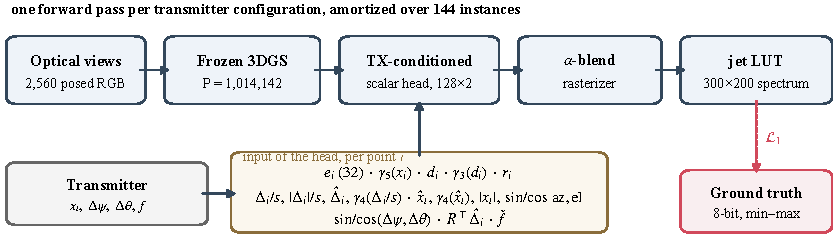
\includegraphics[width=\textwidth]{fig1_pipeline.pdf}
\caption{Overview. Geometry comes from an optical 3DGS and is frozen
($P=1{,}014{,}142$ Gaussians). A per-point embedding, the view ray, and the
transmitter parameters form a 156-dimensional input to a two-layer MLP that
predicts one scalar per Gaussian; the frozen differentiable rasterizer composites
the scalars, and a fixed jet lookup table produces the $300\times200$ spectrum.
Only the head, the embedding and per-point opacity are trained, all of them
across 144 transmitter instances simultaneously. Nothing is optimized at
inference time.}
\label{fig:pipeline}
\end{figure*}

\section{Introduction}

Radio radiance fields estimate spatial channel state information (S-CSI)
densely over a volume rather than at a handful of measured points. RF-3DGS
\cite{rf3dgs} represents a site as 3D Gaussians whose per-point attributes are
optimized against simulated or measured AoA spectra, and renders a spectrum at
an arbitrary receiver pose in milliseconds. Learned radio-map methods
\cite{radiounet} and neural radiance approaches \cite{nerf2} pursue the same
goal with different representations.

All of these formulations share one structural assumption: the model is fitted
to a \emph{particular transmitter}. RF-3DGS attaches the transmitter's
contribution to per-point colours and refits when the transmitter changes;
neural approaches are likewise fitted per source location. In a deployed site this
assumption is the binding constraint. A lobby, hangar, or factory floor hosts
several radios that differ in position, in antenna orientation, and in carrier
frequency, and field engineers routinely re-aim an antenna or change channels.
Refitting per transmitter is expensive, and---more importantly---a site-specific
fit gives no principled answer to the counterfactual question
\emph{what would this room look like if the radio were aimed elsewhere?}

\subsection{Question and scope}
We therefore ask a narrower question than cross-scene generalization: within a
single scene whose geometry is known, can a feed-forward model amortize the fit
over the \emph{transmitter configuration}? Concretely, we condition on a vector
of transmitter parameters $(\Delta\psi, \Delta\theta, f)$---boresight offsets in
yaw and pitch, and carrier frequency---and train one model to render the AoA
spectrum for any of them, including values never seen in training.

\subsection{Why this is not a matter of adding input dimensions}
Three obstacles appear as soon as the problem is posed this way, and each is
addressed in Section~\ref{sec:what}:
\begin{enumerate}
\item \textbf{Confounding.} If every transmitter position carries a single
parameter set, the parameter input is redundant: the model can interpolate
position and ignore it. Generalization to unseen parameters is then untestable.
\item \textbf{Observability.} The dataset normalizes each spectrum to
$[0,1]$ before storage. This silently removes one parameter entirely and
removes the meaning of another, so the modelled parameter vector must be chosen
from what survives the normalization.
\item \textbf{Representation.} Orientation changes \emph{which surfaces are
lit}; frequency changes the coherent phase of every multipath component. A
per-point scalar field can express the first analytically but only
approximately the second, which sets a limit we measure rather than assume.
\end{enumerate}

\subsection{Contributions and findings}
\begin{itemize}
\item A data design (Section~\ref{sec:design}) that decouples transmitter
parameters from position, and a two-stage feasibility gate
(Section~\ref{sec:gate}) that measures whether each parameter axis is
\emph{worth} conditioning on before any large-scale generation or training
budget is spent.
\item A parameter encoding and a frozen-geometry feed-forward architecture
(Section~\ref{sec:method}) whose entire transmitter-conditioned capacity is a
36.7\,k-parameter head plus a per-point embedding.
\item Evidence that unseen-transmitter rendering works inside one scene, with
per-axis honesty about what is and is not established
(Section~\ref{sec:exp}): the main reading improves PSNR by 1.25\,dB over the
published per-scene RF-3DGS, but the two were evaluated under different
generation protocols, and we say so explicitly.
\item A first measurement, to our knowledge, of conditioning a radio radiance
field on array beamforming weights (Section~\ref{sec:w}). We show the axis is
physically feasible and representable, measure the response the current model
realizes ($2.7$--$4.2\%$ of the truth), and localize the bottleneck in base
fidelity rather than in the weight representation.
\end{itemize}

\section{Related Work}
\label{sec:rel}

\paragraph{Radio radiance fields and learned radio maps}
NeRF\textsuperscript{2} \cite{nerf2} models received power as a neural field
over position, conditioned on a source, and regresses path-level quantities.
RF-3DGS \cite{rf3dgs} replaces the coordinate MLP with 3D Gaussians
\cite{3dgs} and targets the full spatial spectrum---AoA, delay, gain of each
multipath component---rather than a scalar power map. GRaF \cite{graf}
trains a generalizable radio radiance field over a set of scenes. Convolutional
radio-map estimators such as RadioUNet \cite{radiounet} predict path loss or
power maps from geometry without a radiance-field parameterization.

\paragraph{Coupled and cross-scene RF Gaussian splatting}
CORF-GS \cite{corfgs} couples optical and radio appearance on shared Gaussian
primitives and quantifies the benefit of joint optimization over a
two-stage (frozen-geometry) baseline. CoRF \cite{corf} separates learned
propagation from analytic array physics and amortizes across scenes using
unordered spectral references.

\paragraph{Array weights as a conditioning variable: an open gap}
Every formulation above treats the transmitter as a \emph{fixed configuration},
and RS--RF-3DGS reconstructs a spectrum from the multipath it measures under
whatever precoder the transmitter happened to use. When the transmitter is an
array, however, its beamforming weights $\mathbf{w}\in\mathbb{C}^{N}$ are a
continuous, physically meaningful, and routinely re-tuned parameter: a base
station re-aims its beam between users within milliseconds. Conditioning a
forward model on $\mathbf{w}$ asks it to render the \emph{same} site under
every beam the array can form. To our knowledge no published radio radiance
field does this, so there is no external baseline for this axis---we report it
as a gap and evaluate it with an internal control instead
(Section~\ref{sec:w}). The closest external anchor is the single-transmitter
setting of Table~\ref{tab:main}, and the two are only shallowly comparable: the
array protocol uses a different transmitter ($4\times4$ instead of $1\times1$),
a different imaging operator (MVDR instead of CBF) and a different instance
set.

\paragraph{Feed-forward 3D reconstruction}
pixelSplat \cite{pixelsplat} and MVSplat \cite{mvsplat} predict 3D Gaussians
from one or two posed images, removing per-scene optimization from the
geometry side. Our setting inherits this: geometry is produced once by an
optical feed-forward/3DGS stage and held fixed.

\paragraph{Positioning}
Cross-scene amortization \cite{corf} and in-scene transmitter amortization are
orthogonal axes. This paper holds the scene fixed and varies the transmitter;
the two could be composed, and we do not attempt that here.

\section{What Can Be Conditioned On}
\label{sec:what}

\begin{figure*}[!t]
\centering
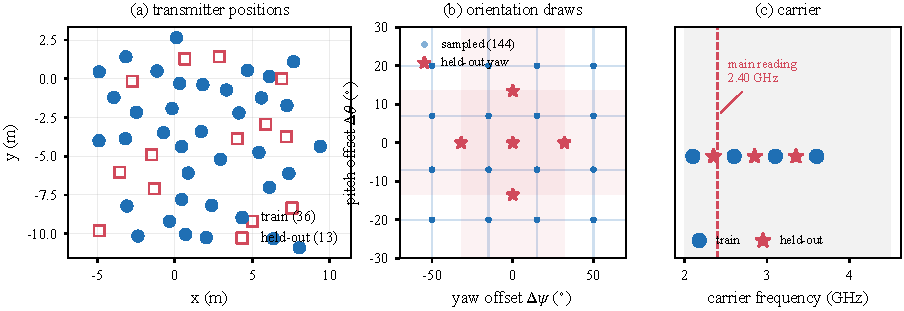
\includegraphics[width=\textwidth]{fig2_design.pdf}
\caption{Data design. (a) Transmitter positions, train versus held out.
(b) Realized orientation draws; shaded bands are held out, so the model is
asked to interpolate. (c) Carrier axis with the declared band shaded, the four
training carriers, three held-out carriers, and the carrier used for the main
reading.}
\label{fig:design}
\end{figure*}

\subsection{Observation model and observability}

Let $\mathbf{x}_t$ be the transmitter position, $\boldsymbol{\Omega}=
(\Delta\psi,\Delta\theta)$ its boresight orientation relative to a scene-facing
base frame, and $f$ the carrier. For a receiver at $\mathbf{p}$ with a
$10\times10$ planar array, the target is a $300\times200$ image
$S(\mathbf{p};\mathbf{x}_t,\boldsymbol{\Omega},f)$ over azimuth and elevation,
obtained by beamforming the multipath components produced by a ray tracer
\cite{sionna,sionnart}. Two properties of this observation model constrain what
may be modelled.

\emph{Per-image min--max normalization removes transmit power exactly.}
The beamformed field is linear in path amplitude, so a transmit power change is a
global multiplier on $S$; after normalizing each image to $[0,1]$, the image is
bit-identical. Power is therefore not a weak or noisy parameter---it is
\emph{unobservable}, and we exclude it rather than fit a coefficient that the
data cannot constrain.

\emph{Polarization is structurally un-learnable here.} The simulator supports a
binary choice (vertical/horizontal). A model can be trained on one value and
tested on the other, but ``an unseen value'' of a two-valued parameter is not a
meaningful generalization target, so we exclude it as well.

What remains is a three-dimensional continuous vector
$(\Delta\psi,\Delta\theta,f)$, all of whose axes admit held-out values.

\subsection{Breaking the parameter--position confound}
\label{sec:design}

The natural way to build such a dataset---one transmitter per position---makes
the parameter input redundant. We instead use a randomized complete block
design (Fig.~\ref{fig:design}): each of 36 training positions receives $n=4$
independent draws of
$(\Delta\psi,\Delta\theta,f)$ from the training domain, giving 144 instances.
Because parameters are drawn independently of position, a position-conditioned
model cannot explain the training data without using the parameter input. We
verify the design numerically by regressing each parameter on the position
coordinates; the maximum $R^2$ over the three axes is $0$.

The parameter domains are chosen so that every axis has a held-out set
\emph{inside} the range spanned by the training values (interpolation, not
extrapolation): yaw offsets $\{-50,-15,15,50\}^\circ$ with held-out
$\{-32,0,32\}^\circ$; pitch offsets $\{-20,-7,7,20\}^\circ$ with held-out
$\{-13.5,0,13.5\}^\circ$; carriers $\{2.1,2.6,3.1,3.6\}$\,GHz with held-out
$\{2.35,2.85,3.35\}$\,GHz inside a declared range of $[2.0,4.5]$\,GHz.
Interpolation measures whether the model represents the parameter, not whether
it dares extrapolate.

\subsection{Encoding}
\label{sec:enc}

\emph{Orientation must be encoded twice.} A circular quantity cannot be fed as
a raw angle: the input would jump at the $0/2\pi$ seam. We encode
$(\sin\Delta\psi,\cos\Delta\psi,\sin\Delta\theta,\cos\Delta\theta)$, and
additionally feed the per-point direction expressed in the transmitter frame,
\begin{equation}
\mathbf{u}_i = R^{\top}\,\widehat{\Delta}_i,\qquad
\widehat{\Delta}_i=\frac{\mathbf{x}_i-\mathbf{x}_t}{\|\mathbf{x}_i-\mathbf{x}_t\|},
\end{equation}
where $R$ is the TR\,38.901 \cite{tr38901} rotation of the transmitter. The
element gain of a directional antenna depends on the angle between the ray and
the boresight \emph{in the antenna frame}; $\mathbf{u}_i$ is the only per-point
quantity that carries this dependence, and it is the term that lets a per-point
scalar field express ``which surfaces are illuminated.''

\emph{Frequency must be normalized over the declared range.} The carrier enters
through the phase $2\pi f\tau_k$ of each path $k$. We feed
$\tilde f = 2(f-f_{\mathrm{lo}})/(f_{\mathrm{hi}}-f_{\mathrm{lo}})-1$ using the
\emph{declared} band $[f_{\mathrm{lo}},f_{\mathrm{hi}}]$, not the observed one,
so that held-out carriers map to interior values of the input rather than
requiring extrapolation, and we do not clip.

\subsection{Why a scalar field rather than a colour field}

The target is a physical intensity. We predict one scalar $u_i\in(0,1)$ per
Gaussian and map it to colour only at render time through a fixed jet lookup
table. This constrains the output to the one-dimensional manifold of realizable
spectra instead of letting the network spend capacity on reproducing the
colormap, and it makes the learned quantity interpretable. In this codebase the
constrained parameterization was consistently stronger than per-point spherical
harmonics or an unconstrained colour MLP on the same geometry; we adopt it as a
design choice and do not claim it as a contribution of this paper.

\section{Method}
\label{sec:method}

Fig.~\ref{fig:pipeline} summarizes the architecture; the rest of this section
details each block.

\subsection{Frozen optical geometry}

The scene provides an optical 3DGS checkpoint fitted to 2{,}560 posed RGB
views. We freeze all geometric and photometric per-point attributes---means,
covariances, rotations and spherical harmonics---and disable densification.
Only three tensors are optimized: a per-point embedding
$e_i\in\mathbb{R}^{32}$ ($32.45$\,M values), per-point opacity
($1.01$\,M values), and the head ($36.7$\,k). The amortization is thus over
\emph{transmitters}, not over scenes: each scene still requires its own
optimization, but that optimization is shared by all transmitters in it.

\subsection{Transmitter-conditioned scalar head}

Table~\ref{tab:inputs} lists the input blocks. The design follows
Section~\ref{sec:enc}; the position blocks are split into a relative part and an
absolute part because they play different roles: $\Delta_i$ and its normalized
form are the quantities that make an \emph{unseen} position extrapolable, while
the absolute $\mathbf{x}_t$ lets the head learn context classes
(near-wall, centre, corridor).

\begin{table}[!t]
\centering
\caption{Input of the scalar head, per Gaussian $i$ (156 dimensions).}
\label{tab:inputs}
\footnotesize
\setlength{\tabcolsep}{3pt}
\begin{tabular}{@{}l>{\raggedright\arraybackslash}p{4.55cm}r@{}}
\toprule
Block & Content & Dim \\
\midrule
Identity & $e_i$ & 32 \\
Position & $\gamma_5(\mathbf{x}_i)$ & 30 \\
View ray & $\mathbf{d}_i$, $\gamma_3(\mathbf{d}_i)$, $r_i$ & 22 \\
Relative TX & $\Delta_i/s$, $|\Delta_i|/s$, $\widehat{\Delta}_i$,
$\gamma_4(\Delta_i/s)$ & 31 \\
Absolute TX & $\widehat{\mathbf{x}}_t$, $\gamma_4(\widehat{\mathbf{x}}_t)$,
$|\mathbf{x}_t|$, $\sin/\cos$ az, el, $\log(1+|\mathbf{x}_t|)$ & 33 \\
Orientation & $\sin/\cos\Delta\psi$, $\sin/\cos\Delta\theta$ & 4 \\
Local dir. & $R^{\top}\widehat{\Delta}_i$ & 3 \\
Carrier & $\tilde f$ & 1 \\
\bottomrule
\end{tabular}
\end{table}

$\gamma_L$ is the Fourier feature of $L$ octaves, $r_i$ the camera-relative
distance, $\widehat{\cdot}$ the scene normalization $(x-c)/s$ with scene scale
$s=8.44$, and $\mathbf{d}_i$ the view ray. The head is $\mathrm{Linear}(156,128)$--ReLU--$\mathrm{Linear}(128,128)$
--ReLU--$\mathrm{Linear}(128,1)$ followed by a sigmoid. Its last layer is
zero-initialized with bias $\mathrm{logit}(0.05)$, so at step zero every
Gaussian carries the same scalar and the model starts from a constant image---a
cold start that makes the first optimization steps comparable across arms.

\subsection{Rendering and objective}

The scalar is replicated to three channels and composited by the frozen
differentiable rasterizer using the dataset's pinhole camera (focal length 150
pixels for a $300\times200$ image, $90^\circ$ field of view). The composite is
quantized to 8 bits and mapped through the fixed jet lookup table. The
objective is an $L_1$ loss between the rendered and target colour-mapped
images, back-propagated through the rasterizer to $e_i$, opacity, and the head.
Geometry never receives gradient.

\subsection{Training}

We train for 180\,k iterations with two views per step, sampling uniformly over
the 144 training instances. Adam is used with a cosine schedule on the head
($8\times10^{-3}\rightarrow8\times10^{-5}$) and a constant
$2.5\times10^{-3}$ on the embedding. A 60\,k-step run from the same
initialization serves as the budget reference.

\subsection{Feasibility gates before spending compute}
\label{sec:gate}

Before generating the full dataset we ran a gated probe at two positions, with
controls that make a negative result readable (Fig.~\ref{fig:gates}).

\begin{figure}[!t]
\centering
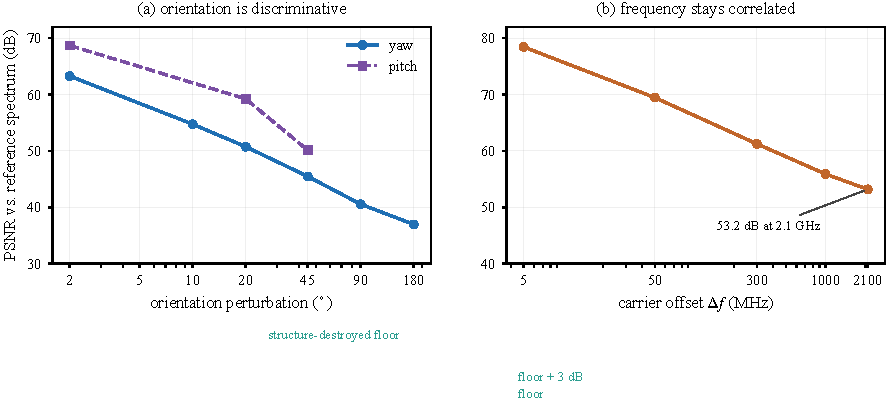
\includegraphics[width=\columnwidth]{fig3_gates.pdf}
\caption{Feasibility gates. (a) Perturbing orientation at a fixed position
produces a monotone decrease in similarity to the reference spectrum, from
$63.3$\,dB at $2^\circ$ to $40.5$\,dB at $90^\circ$; even a $2^\circ$ change is
resolvable. (b) Detuning the carrier from $5$\,MHz to $2.1$\,GHz never reaches
the ``structure destroyed'' threshold (floor $+3$\,dB), so the frequency axis is
learnable over the whole declared band.}
\label{fig:gates}
\end{figure}

\emph{Controls.} Re-running the identical solve reproduces the image to within
one 8-bit level on $1.0\times10^{-7}$ of pixels, and setting the carrier to
4.5\,GHz and back reproduces the 2.4\,GHz image equally exactly---confirming
both solver determinism and that the material model is genuinely frozen
(Section~\ref{sec:protocol} explains why the latter is not automatic). A
spatially permuted image, which destroys all structure while preserving the
histogram, scores 15.34\,dB PSNR; this is our reference for ``the parameter has
erased the image.''

\emph{Orientation} is discriminative and monotone: $63.25$\,dB at $2^\circ$,
$54.72$ at $10^\circ$, $50.72$ at $20^\circ$, $45.46$ at $45^\circ$, $40.53$ at
$90^\circ$, $36.95$ at $180^\circ$, all far above the structural floor.

\emph{Frequency} is the axis the plan flagged as the main risk, because the
phase $2\pi f\tau_k$ decorrelates quickly when delay spreads are tens of
nanoseconds. Measured, it does not: similarity falls from $78.42$\,dB at
$\Delta f=5$\,MHz through $69.44$, $61.23$ and $55.89$ to $53.17$\,dB at
$\Delta f=2.1$\,GHz, never crossing the floor$-3$\,dB threshold. The correlation
width therefore exceeds the entire declared band, and the frequency axis was
kept.

\section{Experiments}
\label{sec:exp}

\subsection{Data and protocol}
\label{sec:protocol}

\begin{table}[!t]
\centering
\caption{Protocol and dataset.}
\label{tab:protocol}
\small
\begin{tabular}{@{}ll@{}}
\toprule
Scene & NIST lobby digital twin ($\approx14\times15$\,m$^2$) \\
Optical & Blender renders, 3{,}200 posed views (2{,}560/640) \\
Image & $300\times200$, $90^\circ$ FoV, 8-bit, per-image min--max \\
Receiver & $10\times10$ planar array, TR\,38.901 pattern \\
Transmitter & $1\times1$ TR\,38.901, vertical polarization \\
Propagation & Sionna RT, max depth 1, specular only \\
Materials & tutorial values at 60\,GHz, frequency callback frozen \\
Carrier & declared $[2.0,4.5]$\,GHz \\
TX positions & 36 train / 13 held out \\
Instances & 36$\times$4 train, 13$\times$4 held out, $+122$ probe \\
Images & 572{,}160 \\
\bottomrule
\end{tabular}
\end{table}

Table~\ref{tab:protocol} summarizes the protocol. Two details matter for
reproducibility. First, the transmitter was changed from an isotropic radiator
to a TR\,38.901 element with a $65^\circ$ azimuth beamwidth: with an isotropic
antenna, rotating the transmitter leaves the image unchanged and the entire
orientation axis is vacuous. Second, Sionna's material objects carry a
frequency-update callback that silently restores the ITU conductivity model when
the scene frequency is set; left in place, changing the carrier would change
\emph{both} propagation and material, and the frequency axis would not be
attributable. We freeze the callback after loading the scene and verify the
freeze with the round-trip probe above.

\subsection{Main reading: unseen position, unseen orientation, unseen carrier}

The main reading is a transmitter at a held-out position, with zero boresight
offset and a 2.40\,GHz carrier. Neither the position nor the orientation value
nor the carrier appears in the training set: $2.40$\,GHz lies in neither the
training set $\{2.1,2.6,3.1,3.6\}$ nor the designated held-out band. It is
scored on the 640 test views shared by all methods, with PSNR, SSIM
\cite{ssim} and LPIPS \cite{lpips}; we treat LPIPS as the perceptual score of
record and report all three everywhere.

\begin{table}[!t]
\centering
\caption{Main reading (640 test views). ``Legacy'' marks rows measured under
the previous generation protocol (isotropic transmitter); see the text.}
\label{tab:main}
\small
\setlength{\tabcolsep}{4pt}
\begin{tabular}{@{}lcccc@{}}
\toprule
Method & Opt. & PSNR$\uparrow$ & SSIM$\uparrow$ & LPIPS$\downarrow$ \\
\midrule
Constant image (floor) & -- & 14.293 & 0.466 & 0.433 \\
RF-3DGS \cite{rf3dgs} (legacy) & per-scene & 14.132 & 0.723 & 0.446 \\
CORF-GS \cite{corfgs} (legacy) & per-scene & 14.633 & 0.755 & 0.403 \\
Prior feed-forward (legacy) & amort. & 11.847 & 0.738 & 0.440 \\
Ours, 60\,k & amort. & 15.314 & 0.766 & 0.403 \\
\textbf{Ours, 180\,k} & amort. & \textbf{15.382} & \textbf{0.764} & 0.404 \\
\bottomrule
\end{tabular}
\end{table}

Table~\ref{tab:main} and Fig.~\ref{fig:main} report the reading. Relative to the
published per-scene RF-3DGS, the feed-forward model gains $1.25$\,dB PSNR,
$0.041$ SSIM and $0.042$ LPIPS while performing no per-transmitter
optimization. Relative to CORF-GS, which couples optical and radio appearance,
we gain $0.75$\,dB PSNR and $0.008$ SSIM, while CORF-GS is marginally better on
LPIPS ($0.4029$ vs $0.4040$).

\begin{figure}[!t]
\centering
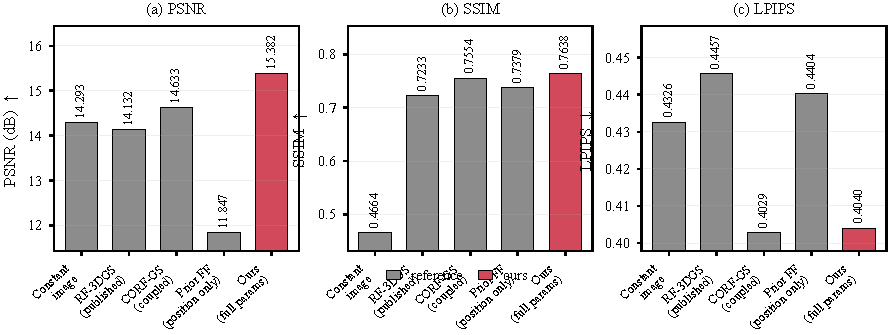
\includegraphics[width=\columnwidth]{fig5_main.pdf}
\caption{Main reading. Grey bars are references; the red bar is the
feed-forward model with full parameter conditioning. The constant-image floor
is the per-view mean of the training ground truth---the strongest predictor
that uses no transmitter information at all.}
\label{fig:main}
\end{figure}

\emph{These comparisons are indicative, not exact.} The reference rows were
produced under the previous generation protocol, which used an isotropic
transmitter. We measured the discrepancy directly: swapping the isotropic
radiator for the TR\,38.901 element changes the target image by $43.0$\,dB PSNR,
i.e.\ an RMS error of $1.8$ grey levels out of 255, whereas the methods' own
errors are of order 50--65 grey levels. In quadrature this moves a reading by
$0.005$\,dB. We therefore treat the numbers as comparable to within
$\pm0.1$\,dB and do not interpret differences below that. The prior
feed-forward row differs additionally in its training set (49 transmitters, one
configuration each, versus 144 instances here); we do not decompose the
$3.53$\,dB gap between it and ours.

\emph{What the PSNR does and does not say.} AoA spectra are dominated by a
static background: a constant image built from the training ground truth already
scores $14.29$\,dB. Against that floor the PSNR margin is $1.09$\,dB, while
SSIM rises from $0.466$ to $0.764$ and LPIPS falls from $0.433$ to $0.404$. The
perceptual and structural gains are much larger than the PSNR gain, and we
regard the PSNR margin over the constant image as the weaker evidence.

\subsection{Held-out positions}

The second reading isolates position generalization: 52 instances generated from
13 held-out positions, four parameter draws each, all parameters inside the
training domain.

\begin{table}[!t]
\centering
\caption{Held-out positions, 52 instances (13 positions $\times$ 4 draws).
$\Delta$ is $180$\,k minus $60$\,k; SE is the standard error of the paired
difference. The last column counts instances where the 180\,k run has the
larger value (LPIPS is lower-better, so fewer is better there).}
\label{tab:holdout}
\small
\setlength{\tabcolsep}{4pt}
\begin{tabular}{@{}lccccc@{}}
\toprule
Metric & 60\,k & 180\,k & $\Delta$ & SE & higher \\
\midrule
PSNR & 15.752 & 15.879 & $+0.127$ & 0.021 & 44/52 \\
SSIM & 0.7957 & 0.7953 & $-0.00047$ & 0.00019 & 19/52 \\
LPIPS & 0.3682 & 0.3683 & $+0.00015$ & 0.00026 & 22/52 \\
\bottomrule
\end{tabular}
\end{table}

\begin{figure}[!t]
\centering
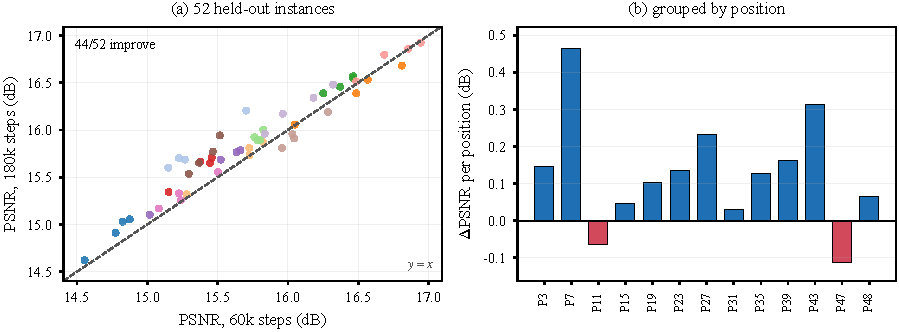
\includegraphics[width=\columnwidth]{fig6_holdout.pdf}
\caption{Held-out positions. (a) Per-instance PSNR at 60\,k and 180\,k steps;
points above the diagonal improve with the longer schedule. (b) The same
difference grouped by position (four draws averaged); 11 of 13 positions
improve. The gain is small but consistent in sign.}
\label{fig:holdout}
\end{figure}

Table~\ref{tab:holdout} and Fig.~\ref{fig:holdout} show that the longer
schedule buys PSNR reliably ($+0.127$\,dB, $t=6.0$ at the instance level and
$+0.127\pm0.042$\,dB when positions are treated as the unit of analysis) but
slightly \emph{costs} SSIM ($-0.00047$, $t=-2.5$) and leaves LPIPS unchanged.
We report this rather than only the PSNR gain: at this scale of difference the
three metrics do not move together, and the honest summary is that the budget
is spent on spectral accuracy in the PSNR sense.

\subsection{Qualitative comparison}

Fig.~\ref{fig:qual} places ground truth, the released RF-3DGS render and ours on
four test views. The most visible difference is not peak localization---all
methods place the dominant lobe---but the low-contrast background structure,
which the per-scene baseline smooths out.

\begin{figure*}[!t]
\centering
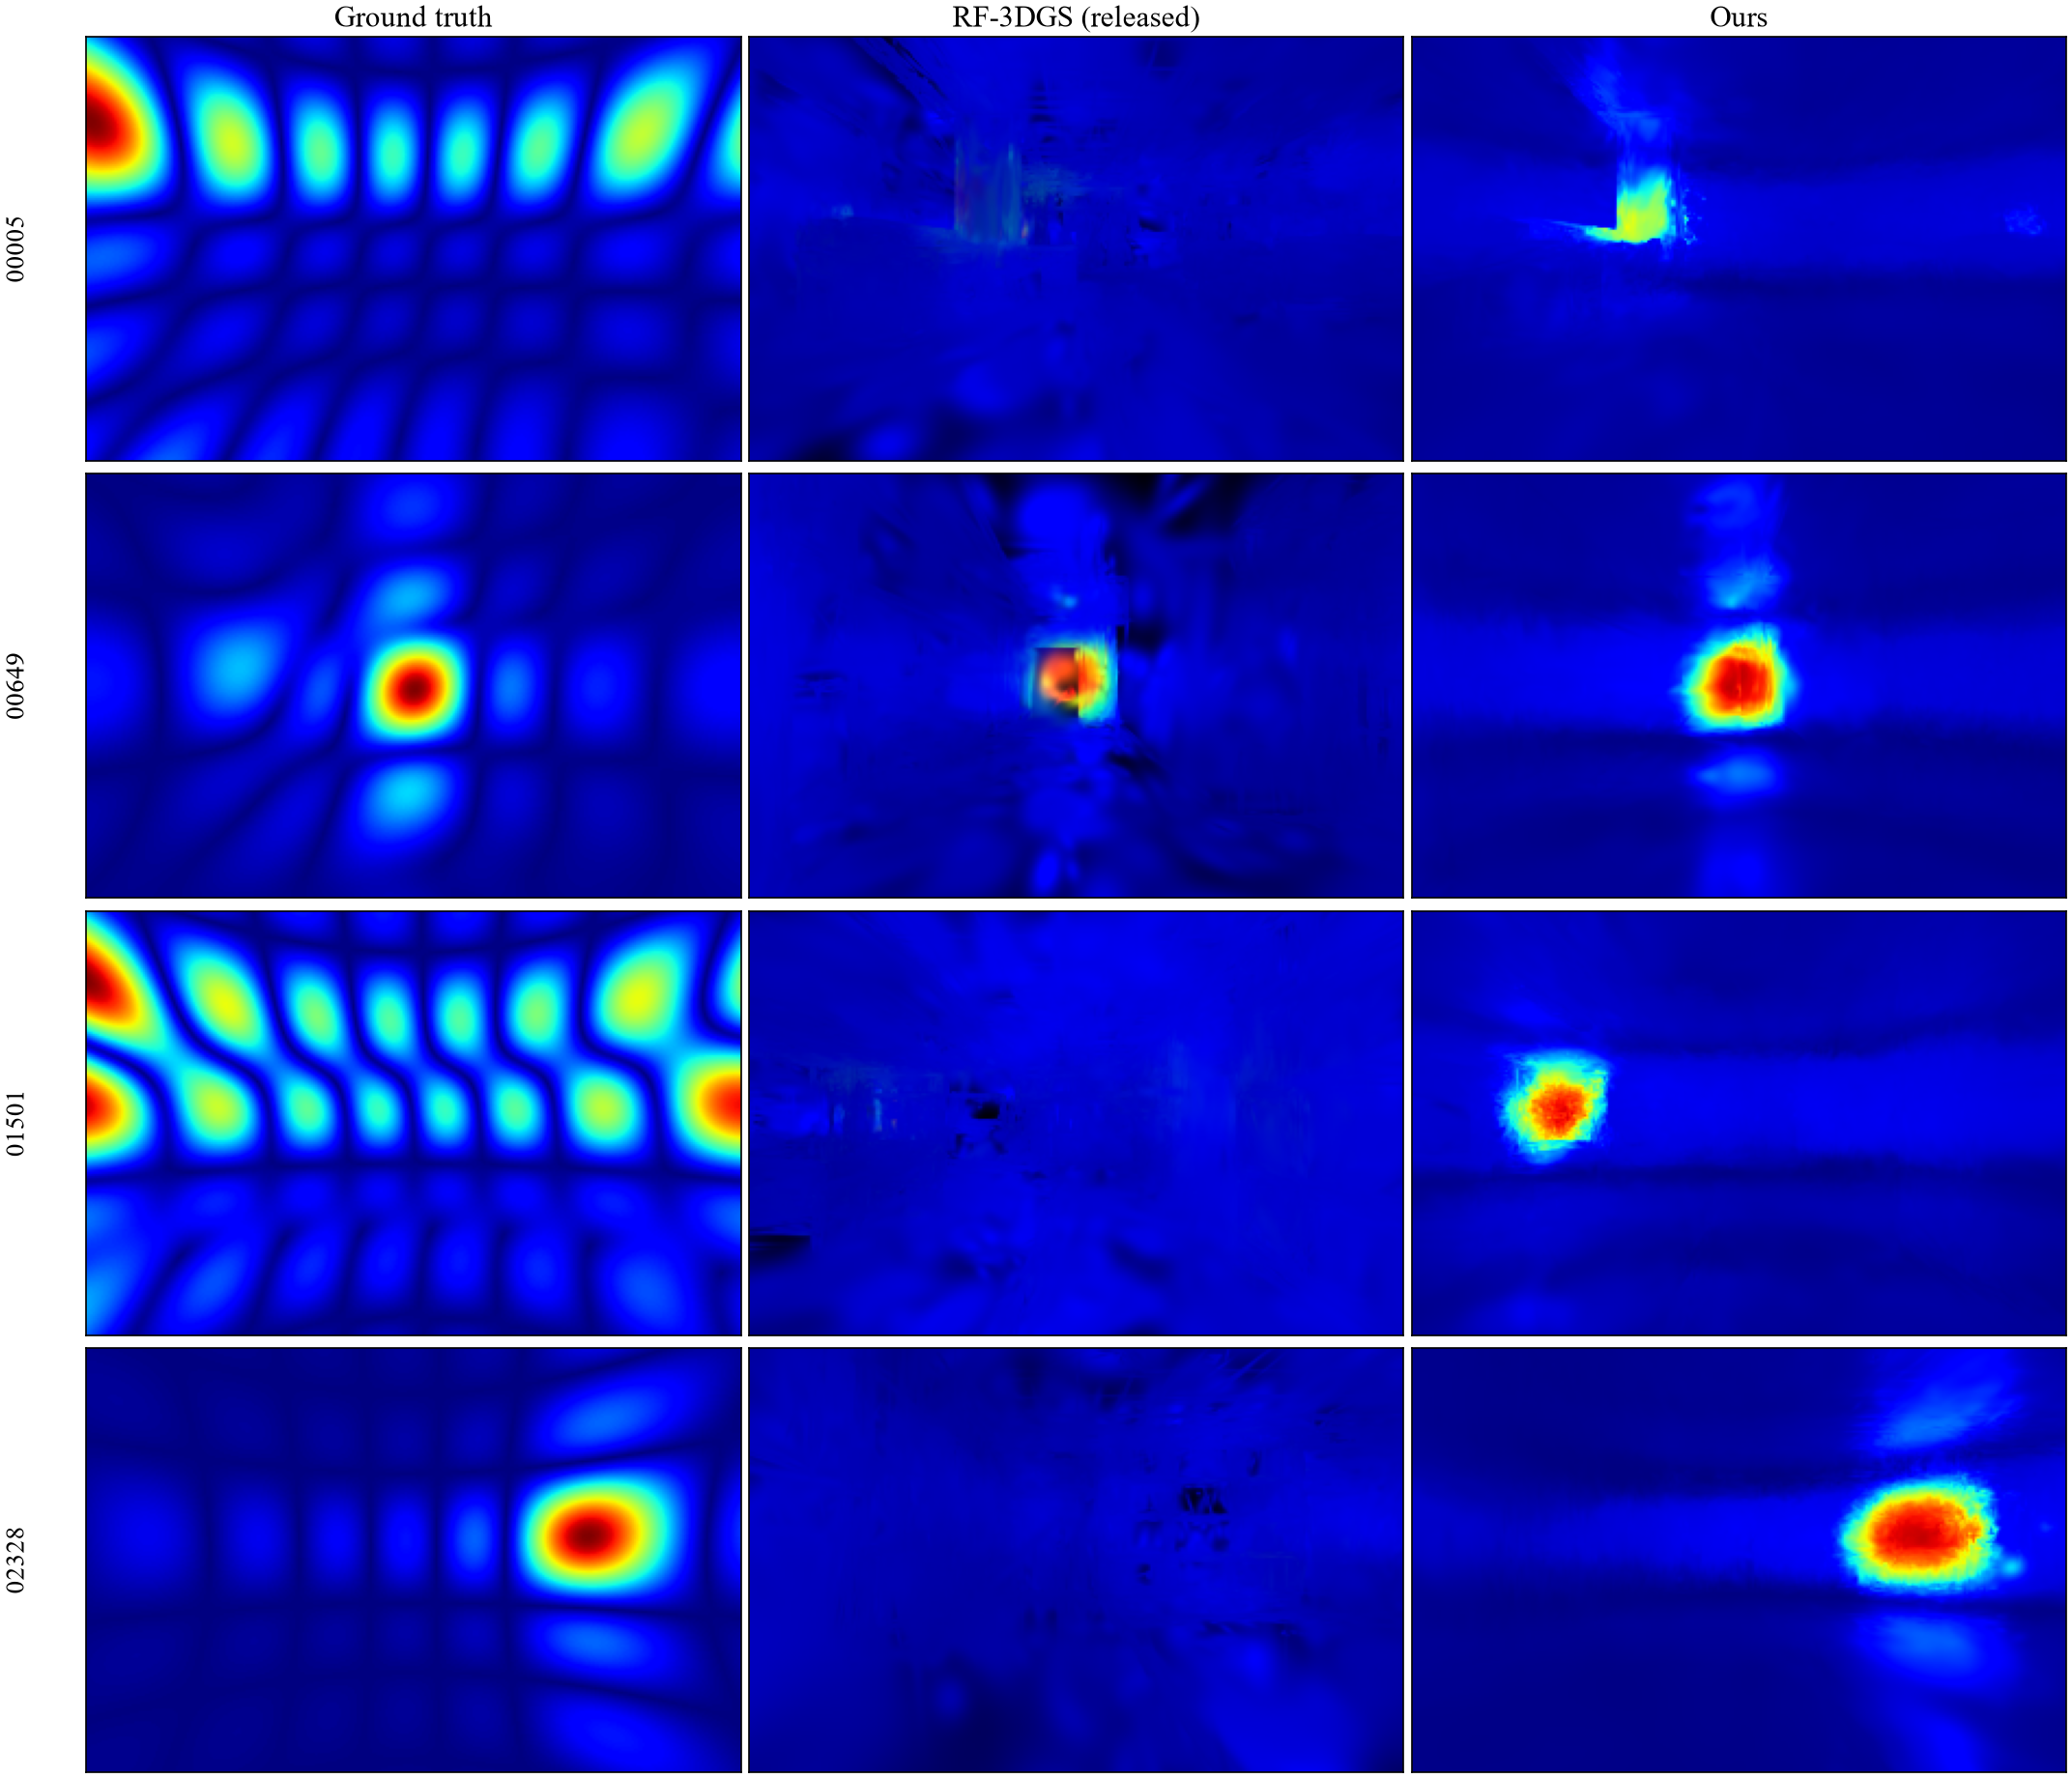
\includegraphics[width=\textwidth]{fig4_qual.png}
\caption{Qualitative comparison on the main reading (instance 317). Columns:
ground truth, released RF-3DGS render (legacy protocol, included as a visual
reference), and our feed-forward render. Jets are the dataset's fixed colour
map; brightness is not comparable across rows.}
\label{fig:qual}
\end{figure*}

\subsection{Second channel model: regularized MVDR}
\label{sec:mvdr}

The protocol above renders a conventional beamforming (CBF) spectrum from a
handful of specular paths. To test whether the conditioning mechanism is tied to
that particular imaging operator, we regenerated the same 318 transmitter
instances with regularized MVDR (Capon) beamforming:
$p=1/|\mathbf{a}^{H}R^{-1}\mathbf{a}|$ with $R$ the array covariance, diagonal
loading $\varepsilon=0.01$ for well-posedness, a $0.1$\,ns delay grid, and
diffuse scattering enabled---about $1.6\times10^{5}$ multipath components per
solve instead of roughly six. MVDR is not linear in the array response:
changing the transmitter configuration changes $R$ itself and therefore the
adaptive weights, so the field-to-image map is appreciably more nonlinear than
that of CBF. Training used the same 144 instances, the same frozen optical
geometry and the same 180\,k schedule as the main run.

\begin{table}[!t]
\centering
\caption{Regularized MVDR channel model (second imaging operator). The floor row
is measured on the main reading's ground truth only.}
\label{tab:mvdr}
\small
\setlength{\tabcolsep}{4pt}
\begin{tabular}{@{}lccc@{}}
\toprule
Setting & PSNR$\uparrow$ & SSIM$\uparrow$ & LPIPS$\downarrow$ \\
\midrule
Constant image (floor, main reading) & 11.381 & 0.411 & 0.506 \\
Held-out positions (52) & 13.795 & 0.713 & 0.432 \\
\textbf{Main reading} & \textbf{14.209} & \textbf{0.718} & \textbf{0.436} \\
\bottomrule
\end{tabular}
\end{table}

\begin{figure}[!t]
\centering
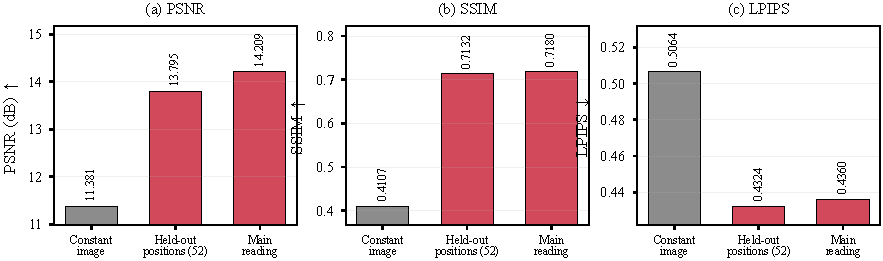
\includegraphics[width=\columnwidth]{fig7_mvdr.pdf}
\caption{MVDR channel model. Grey bar: constant-image floor on the main reading's
ground truth. Red bars: the feed-forward model. Read against the floor, not
against Table~\ref{tab:main}.}
\label{fig:mvdr}
\end{figure}

Three things change when the imaging operator changes. First, the absolute
numbers are not comparable with Table~\ref{tab:main}: under MVDR the
constant-image floor itself falls to $11.38$\,dB / $0.411$ / $0.506$, i.e.\ the
target is intrinsically harder and its LPIPS floor sits $0.07$ above the CBF one.
Second, the margin over that floor is \emph{larger}, not smaller: $+2.83$\,dB
PSNR, $+0.307$ SSIM and $-0.070$ LPIPS, against $+1.09$\,dB, $+0.298$ and
$-0.029$ on CBF. Third, the held-out-position group behaves as it did on CBF
($13.795$\,dB, slightly below the main reading), so the position-generalization
conclusion is unchanged.

We read this arm as support for the claim that what carries over is the
conditioning mechanism, not a property of one rendering operator. Two caveats
bound that reading: this arm has no 60\,k baseline and no external reference, and
the CBF-format references in Table~\ref{tab:main} are on a different axis and are
deliberately not reproduced here.

\section{Array-Level Conditioning: Beamforming Weights $\mathbf{w}$}
\label{sec:w}

The transmitter parameters above are properties of a single antenna element.
We now push the same mechanism one level down---or rather up---the chain, and
condition the model on the \emph{beamforming weights} of an array transmitter.
This is the axis on which the literature is silent
(Section~\ref{sec:rel}): a site is usually served by an array whose precoder is
recomputed continuously, and no published radiance field renders the spectrum
for arbitrary $\mathbf{w}$.

\subsection{Protocol and what the normalization hides}

We regenerate the scene with a $4\times4$ TR\,38.901 transmit array and the
regularized MVDR operator of Section~\ref{sec:mvdr}, giving 354 instances. The
model is trained on the base instances and evaluated on 36 derived instances
(ids 318--353) whose weights never appear in training, each with 640 test
views; all metrics are in the jet delivery domain.

One property of the observation model bounds what can be claimed.
Each image is min--max normalized, while a beamforming weight scales the
transmit power by 17--27\,dB relative to a uniform precoder (median $+18.6$\,dB
under MVDR). The normalization removes that gain completely, so $\mathbf{w}$ is
observable only through the \emph{spatial shape} it imprints. Array-gain
metrics are therefore out of reach without storing per-image
$v_{\min}/v_{\max}$, and we report none.

\subsection{Feasibility of the axis}

Probes on this protocol confirm the axis is real and, importantly, learnable:
swapping $\mathbf{w}$ for a uniform precoder moves the image by a median of
$17.41$\,dB ($p_{10}=15.10$), an approximation using only per-path real gains
reproduces the exact image to $29.52$\,dB ($p_{10}=24.55$, worst $18.09$), and
the image difference is low-pass in beam angle---$26.09$\,dB at $5$--$10^\circ$
separation, saturating at $16.29$\,dB beyond $80^\circ$ against a
pixel-permutation floor of $13.10$\,dB. A per-point scalar field can therefore
carry the effect, and the angular scale to resolve ($10$--$20^\circ$) is coarse.

\subsection{Three arms}

We compare two ways of injecting $\mathbf{w}$ with a control that does not see
it at all (Table~\ref{tab:w}, Fig.~\ref{fig:w}). All three share the frozen
geometry, the schedule and every hyperparameter.

\begin{table}[!t]
\centering
\caption{Beamforming-weight conditioning on 36 held-out $\mathbf{w}$
(640 test views each). The bottom block is computed from ground truth only and
is not a model: it bounds what ``ignoring $\mathbf{w}$'' can achieve.}
\label{tab:w}
\small
\setlength{\tabcolsep}{4pt}
\begin{tabular}{@{}lccc@{}}
\toprule
Setting & PSNR$\uparrow$ & SSIM$\uparrow$ & LPIPS$\downarrow$ \\
\midrule
Complex $\mathbf{w}$, $\lambda_p=0$ & 11.557 & 0.7020 & 0.4627 \\
Complex $\mathbf{w}$, $+\mathcal{L}_{\mathrm{LPIPS}}$ & 11.712 & 0.6871 & 0.4621 \\
\textbf{w-blind (control)} & \textbf{12.209} & \textbf{0.6894} & \textbf{0.4455} \\
\midrule
\multicolumn{4}{@{}l}{\emph{Reference floors from ground truth only}}\\
Same-position training-$\mathbf{w}$ prior & 13.534 & 0.6498 & 0.2902 \\
Sibling instance (other $\mathbf{w}$) & 12.460 & 0.6946 & 0.2877 \\
Same-position median & 12.723 & 0.6943 & 0.2959 \\
\bottomrule
\end{tabular}
\end{table}

\begin{figure}[!t]
\centering
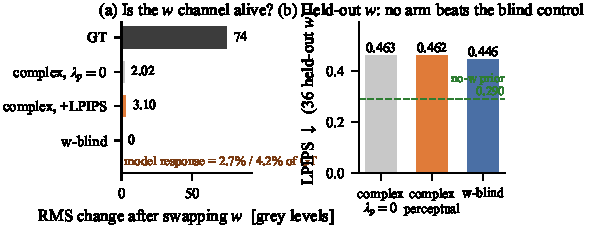
\includegraphics[width=\columnwidth]{fig8_w_channel.pdf}
\caption{Array-weight conditioning. (a) RMS change of the rendered image when
the instance's $\mathbf{w}$ is replaced by a same-position weight from the
training domain, in grey levels (0--255). The control is exactly zero, so the
exotic arms' 2--3 levels are a real, non-degenerate response---but it is
$2.7$--$4.2\%$ of the ground-truth effect. (b) LPIPS on the 36 held-out
weights; none of the $\mathbf{w}$-aware arms reaches the blind control, and
all remain far above the ground-truth prior floor.}
\label{fig:w}
\end{figure}

Two readings follow. First, the conditioning path is \emph{live}: swapping
$\mathbf{w}$ changes the model's rendering by $2.02$ and $3.10$ grey levels in
the two arms, against exactly $0.000$ for the blind control, whose zero was
verified on the same probe where the answer is known. Second, the response is
\emph{weak}: the ground truth moves by $74.50$ grey levels under the same swap,
so the model realizes $2.7$--$4.2\%$ of the effect, and the blind control still
wins by $0.50$\,dB PSNR and $0.0166$ LPIPS. In other words, the model does
generalize to unseen $\mathbf{w}$ in a qualitative sense---the output moves in
the right direction and by an amount that scales with the weight change---but
not yet in a quantitative one.

\subsection{Why the effect is small, and what it would take}

The deficit is not in the weight representation. A shared 16-dimensional
complex field of the form $c_p(\mathbf{w})=\sum_n \overline{w_n}\,s_{pn}$
generalizes to arbitrary $\mathbf{w}$ by construction and trails a free
per-instance complex field by only $0.76$\,dB. The binding constraint is the
\emph{base} rendering fidelity. On the paired $\mathbf{w}$ dataset the
pooled $u$-domain effect of changing $\mathbf{w}$ is an RMSE of $0.093$
($\approx20.3$\,dB), while the model's base error is $0.106$--$0.160$: the
signal is smaller than or comparable to the error it must be seen through.
Composing the two quadratically, a model that rendered $\mathbf{w}$
\emph{perfectly} would gain only
$20\log_{10}(0.1508/0.1060)=3.06$\,dB (or $2.05$\,dB using the global effect
mean $0.0926$), and the 13-epoch angular run confirms the same magnitude
($+0.5$\,dB). Any $\mathbf{w}$ arm therefore differs from its control by
amounts of the order of the $0.365$\,dB noise floor, which is exactly what
Table~\ref{tab:w} shows. Raising this ceiling requires improving base fidelity
first; we state that as the principal open problem of this axis rather than
reporting further representation variants.

\subsection{Data and code availability}

The project is released as \emph{w-RFGS}. The repository contains the
generator, the training and evaluation code, the instance tables and the
per-run configuration files; the rendered spectra (572{,}160 images for the
CBF protocol, plus the MVDR and $\mathbf{w}$ variants, several GB in total) are
distributed as a separate archive rather than committed, with a SHA-256
checksum listed alongside it. Every generated image is reproducible from
Table~\ref{tab:protocol}: the public NIST lobby digital twin is traced with
Sionna RT under the stated transmitter, receiver, material and normalization
settings, and the instance tables fix the parameter draws. The download
locations and the exact commands are kept in the repository README
(\texttt{docs/DATASETS.md}) so that they stay current with the code.

\section{Discussion and Limitations}
\label{sec:disc}

\paragraph{Single scene.} Every number here comes from one room. The
amortization is over transmitters within that room; nothing in the experiments
supports a claim about a new room. Composing this with cross-scene
amortization \cite{corf} is the natural next step and is not attempted.

\paragraph{One transmitter at a time.} We model a single active transmitter and
normalize each spectrum. Simultaneous transmitters would superpose in the field
but the per-image normalization destroys the relative scale between them, so
the current pipeline cannot represent the mixture without a separate mechanism
for relative power. This is a real constraint of the observation model, not an
implementation gap.

\paragraph{Per-axis ablations are not separable.} We do not report arms that
remove one parameter at a time. The gate data explain why: a $45^\circ$ yaw
change moves the target by $45.5$\,dB PSNR while moving the transmitter between
two positions moves it by only $14$--$15$\,dB, i.e.\ the parameter effect is
about three orders of magnitude smaller in image MSE than the position effect.
Against that scale, differences between per-axis arms would be dominated by
optimization noise, and reporting them as wins or losses would be
over-claiming. What the data do support is that training on randomized
parameter draws does not degrade position generalization (Table~\ref{tab:holdout})
and that the joint unseen-position/unseen-parameter case is rendered
competitively (Table~\ref{tab:main}).

\paragraph{Array weights are representable, not yet exploited.}
Section~\ref{sec:w} shows a live but weak $\mathbf{w}$ channel: the model
responds to a weight it has never seen, at $2.7$--$4.2\%$ of the ground-truth
effect, and loses to a control that ignores $\mathbf{w}$. We do not read this
as evidence against the axis---the ceiling imposed by base fidelity is
$2$--$3$\,dB, larger than any effect we could currently resolve---but it does
mean that a $\mathbf{w}$-conditioned model is not yet a usable replacement for
per-precoder fitting.

\paragraph{Cross-protocol references.} As stated in Section~\ref{sec:exp}, the
published and legacy rows were generated with a different transmitter antenna.
We quantified the discrepancy and argued it is below our resolution, but it
remains a caveat rather than a controlled comparison.

\section{Conclusion}

A radio radiance field can be amortized over transmitter configurations inside a
scene, not only over receiver poses. The ingredients that made it work were
mostly about what to leave out: exclude parameters the normalization makes
unobservable, remove the parameter--position confound in the data, encode
orientation where the antenna physics acts (the per-point direction in the
transmitter frame) and frequency over the declared rather than the observed
band, and constrain the output to a scalar field so the network models the
physics rather than the colormap. With geometry frozen from an optical 3DGS and
only a 36.7\,k-parameter head trained across 144 transmitter instances, an
unseen position with an unseen orientation and carrier is rendered in one
forward pass at 15.38\,dB PSNR / 0.764 SSIM / 0.404 LPIPS. The remaining
weaknesses are stated in Section~\ref{sec:disc}: one scene, one transmitter at a
time, and external comparisons that are indicative rather than exact. The same
mechanism extends to the beamforming weights of an array transmitter, where we
find a live but weak channel: unseen weights change the rendering, but only by
a few percent of the true effect, and the binding constraint is base fidelity
rather than the weight representation.

\bibliographystyle{IEEEtran}
\bibliography{refs}

\end{document}
